%%**************************************************************
%% Vorlage fuer Bachelorarbeiten (o.ä.) der DHBW
%%
%% Autor: Tobias Dreher, Yves Fischer
%% Datum: 06.07.2011
%%
%% Autor: Michael Gruben
%% Datum: 15.05.2013
%%
%% Autor: Markus Barthel
%% Datum: 22.08.2014
%%**************************************************************

%!TEX root = ../dokumentation.tex

%
% Nahezu alle Einstellungen koennen hier getaetigt werden
%

\RequirePackage[l2tabu, orthodox]{nag}	% weist in Commandozeile bzw. log auf veraltete LaTeX Syntax hin

\documentclass[%
	pdftex,
	oneside,			% Einseitiger Druck.
	12pt,				% Schriftgroesse
	parskip=half,		% Halbe Zeile Abstand zwischen Absätzen.
%	topmargin = 10pt,	% Abstand Seitenrand (Std:1in) zu Kopfzeile [laut log: unused]
	headheight = 12pt,	% Höhe der Kopfzeile
%	headsep = 30pt,	% Abstand zwischen Kopfzeile und Text Body  [laut log: unused]
	headsepline,		% Linie nach Kopfzeile.
	footsepline,		% Linie vor Fusszeile.
	footheight = 16pt,	% Höhe der Fusszeile
	abstracton,		% Abstract Überschriften
	DIV=calc,		% Satzspiegel berechnen
	BCOR=8mm,		% Bindekorrektur links: 8mm
	headinclude=false,	% Kopfzeile nicht in den Satzspiegel einbeziehen
	footinclude=false,	% Fußzeile nicht in den Satzspiegel einbeziehen
	listof=totoc,		% Abbildungs-/ Tabellenverzeichnis im Inhaltsverzeichnis darstellen
	toc=bibliography,	% Literaturverzeichnis im Inhaltsverzeichnis darstellen
]{scrreprt}	% Koma-Script report-Klasse, fuer laengere Bachelorarbeiten alternativ auch: scrbook

% Einstellungen laden
\usepackage{xstring}
\usepackage[utf8]{inputenc}
\usepackage[T1]{fontenc}

\newcommand{\einstellung}[1]{%
  \expandafter\newcommand\csname #1\endcsname{}
  \expandafter\newcommand\csname setze#1\endcsname[1]{\expandafter\renewcommand\csname#1\endcsname{##1}}
}
\newcommand{\langstr}[1]{\einstellung{lang#1}}

\einstellung{matrikelnr}
\einstellung{titel}
\einstellung{kurs}
\einstellung{datumAbgabe}
\einstellung{firma}
\einstellung{firmenort}
\einstellung{abgabeort}
\einstellung{abschluss}
\einstellung{studiengang}
\einstellung{dhbw}
\einstellung{betreuer}
\einstellung{gutachter}
\einstellung{zeitraum}
\einstellung{arbeit}
\einstellung{autor}
\einstellung{sprache}
\einstellung{schriftart}
\einstellung{seitenrand}
\einstellung{kapitelabstand}
\einstellung{spaltenabstand}
\einstellung{zeilenabstand}
\einstellung{zitierstil}
 % verfügbare Einstellungen
%%%%%%%%%%%%%%%%%%%%%%%%%%%%%%%%%%%%%%%%%%%%%%%%%%%%%%%%%%%%%%%%%%%%%%%%%%%%%%%
%                                   Einstellungen
%
% Hier können alle relevanten Einstellungen für diese Arbeit gesetzt werden.
% Dazu gehören Angaben u.a. über den Autor sowie Formatierungen.
%
%
%%%%%%%%%%%%%%%%%%%%%%%%%%%%%%%%%%%%%%%%%%%%%%%%%%%%%%%%%%%%%%%%%%%%%%%%%%%%%%%


%%%%%%%%%%%%%%%%%%%%%%%%%%%%%%%%%%%% Sprache %%%%%%%%%%%%%%%%%%%%%%%%%%%%%%%%%%%
%% Aktuell sind Deutsch und Englisch unterstützt.
%% Es werden nicht nur alle vom Dokument erzeugten Texte in
%% der entsprechenden Sprache angezeigt, sondern auch weitere
%% Aspekte angepasst, wie z.B. die Anführungszeichen und
%% Datumsformate.
\setzesprache{de} % oder en
%%%%%%%%%%%%%%%%%%%%%%%%%%%%%%%%%%%%%%%%%%%%%%%%%%%%%%%%%%%%%%%%%%%%%%%%%%%%%%%%

%%%%%%%%%%%%%%%%%%%%%%%%%%%%%%%%%%% Angaben  %%%%%%%%%%%%%%%%%%%%%%%%%%%%%%%%%%%
%% Die meisten der folgenden Daten werden auf dem
%% Deckblatt angezeigt, einige auch im weiteren Verlauf
%% des Dokuments.
\setzematrikelnr{1234510}
\setzekurs{TINF2014MI}
\setzetitel{Dies ist der Titel der Bachelorarbeit und bitte ohne Rechtschreibfehler}
\setzedatumAbgabe{Septemper 2017}
\setzefirma{Firma GmbH}
\setzefirmenort{Firmenort}
\setzeabgabeort{Abgabeort}
\setzeabschluss{Bachelor of Science}
%Für MI immer \setzeabschluss{Bachelor of Science}
%Für IA/IM bis INF2016: \setzeabschluss{Bachelor of Engineering}
%ab INF2017 generell \setzeabschluss{Bachelor of Science}
\setzestudiengang{Informatik}
\setzedhbw{Heidenheim}
\setzebetreuer{Dipl.-Ing.~(FH) Peter Pan}
\setzegutachter{Prof. Dr.\ Rolf Assfalg}
\setzezeitraum{12 Wochen}
\setzearbeit{Bachelorarbeit}
\setzeautor{Michael Lustig}
%%%%%%%%%%%%%%%%%%%%%%%%%%%%%%%%%%%%%%%%%%%%%%%%%%%%%%%%%%%%%%%%%%%%%%%%%%%%%%%%

%%%%%%%%%%%%%%%%%%%%%%%%%%%% Literaturverzeichnis %%%%%%%%%%%%%%%%%%%%%%%%%%%%%%
%% Bei Fehlern während der Verarbeitung bitte in ads/header.tex bei der
%% Einbindung des Pakets biblatex (ungefähr ab Zeile 110,
%% einmal für jede Sprache), biber in bibtex ändern.
\newcommand{\ladeliteratur}{%
\addbibresource{bibliographie.bib}
%\addbibresource{weitereDatei.bib}
}
%% Zitierstil
%% siehe: http://ctan.mirrorcatalogs.com/macros/latex/contrib/biblatex/doc/biblatex.pdf (3.3.1 Citation Styles)
%% mögliche Werte z.B numeric-comp, alphabetic, 
%% Weniger gut: authoryear, alphabetic-verb, 
\setzezitierstil{alphabetic-verb}
%%%%%%%%%%%%%%%%%%%%%%%%%%%%%%%%%%%%%%%%%%%%%%%%%%%%%%%%%%%%%%%%%%%%%%%%%%%%%%%%

%%%%%%%%%%%%%%%%%%%%%%%%%%%%%%%%% Layout %%%%%%%%%%%%%%%%%%%%%%%%%%%%%%%%%%%%%%%
%% Verschiedene Schriftarten
% laut nag Warnung: palatino obsolete, use mathpazo, helvet (option scaled=.95), courier instead
\setzeschriftart{lmodern} % palatino oder goudysans, lmodern, libertine

%% Paket um Textteile drehen zu können
%\usepackage{rotating}
%% Paket um Seite im Querformat anzuzeigen
%\usepackage{lscape}

%% Seitenränder
\setzeseitenrand{2.5cm}

%% Abstand vor Kapitelüberschriften zum oberen Seitenrand
\setzekapitelabstand{20pt}

%% Spaltenabstand
\setzespaltenabstand{10pt}
%%Zeilenabstand innerhalb einer Tabelle
\setzezeilenabstand{1.5}
%%%%%%%%%%%%%%%%%%%%%%%%%%%%%%%%%%%%%%%%%%%%%%%%%%%%%%%%%%%%%%%%%%%%%%%%%%%%%%%%

%%%%%%%%%%%%%%%%%%%%%%%%%%%%% Verschiedenes  %%%%%%%%%%%%%%%%%%%%%%%%%%%%%%%%%%%
%% Farben (Angabe in HTML-Notation mit großen Buchstaben)
\newcommand{\ladefarben}{%
	\definecolor{LinkColor}{HTML}{00007A}
	\definecolor{ListingBackground}{HTML}{FCF7DE}
}
%% Mathematikpakete benutzen (Pakete aktivieren)
%\usepackage{amsmath}
%\usepackage{amssymb}

%% Programmiersprachen Highlighting (Listings)
\newcommand{\listingsettings}{%
	\lstset{%
		language=Java,			% Standardsprache des Quellcodes
		numbers=left,			% Zeilennummern links
		stepnumber=1,			% Jede Zeile nummerieren.
		numbersep=5pt,			% 5pt Abstand zum Quellcode
		numberstyle=\tiny,		% Zeichengrösse 'tiny' für die Nummern.
		breaklines=true,		% Zeilen umbrechen wenn notwendig.
		breakautoindent=true,	% Nach dem Zeilenumbruch Zeile einrücken.
		postbreak=\space,		% Bei Leerzeichen umbrechen.
		tabsize=2,				% Tabulatorgrösse 2
		basicstyle=\ttfamily\footnotesize, % Nichtproportionale Schrift, klein für den Quellcode
		showspaces=false,		% Leerzeichen nicht anzeigen.
		showstringspaces=false,	% Leerzeichen auch in Strings ('') nicht anzeigen.
		extendedchars=true,		% Alle Zeichen vom Latin1 Zeichensatz anzeigen.
		captionpos=b,			% sets the caption-position to bottom
		backgroundcolor=\color{ListingBackground}, % Hintergrundfarbe des Quellcodes setzen.
		xleftmargin=0pt,		% Rand links
		xrightmargin=0pt,		% Rand rechts
		frame=single,			% Rahmen an
		frameround=ffff,
		rulecolor=\color{darkgray},	% Rahmenfarbe
		fillcolor=\color{ListingBackground},
		keywordstyle=\color[rgb]{0.133,0.133,0.6},
		commentstyle=\color[rgb]{0.133,0.545,0.133},
		stringstyle=\color[rgb]{0.627,0.126,0.941}
	}
}
%%%%%%%%%%%%%%%%%%%%%%%%%%%%%%%%%%%%%%%%%%%%%%%%%%%%%%%%%%%%%%%%%%%%%%%%%%%%%%%%

%%%%%%%%%%%%%%%%%%%%%%%%%%%%%%%% Eigenes %%%%%%%%%%%%%%%%%%%%%%%%%%%%%%%%%%%%%%%
%% Hier können Ergänzungen zur Präambel vorgenommen werden (eigene Pakete, Einstellungen)



 % lese Einstellungen

\newcommand{\iflang}[2]{%
  \IfStrEq{\sprache}{#1}{#2}{}
}

\langstr{abkverz}
\langstr{anhang}
\langstr{glossar}
\langstr{deckblattabschlusshinleitung}
\langstr{artikelstudiengang}
\langstr{studiengang}
\langstr{anderdh}
\langstr{von}
\langstr{dbbearbeitungszeit}
\langstr{dbmatriknr}
\langstr{dbkurs}
\langstr{dbfirma}
\langstr{dbbetreuer}
\langstr{dbgutachter}
\langstr{sperrvermerk}
\langstr{erklaerung}
\langstr{abstract}
\langstr{listingname}
\langstr{listlistingname}
\langstr{listingautorefname}
 % verfügbare Strings
\input{lang/\sprache} % Übersetzung einlesen

% Einstellung der Sprache des Paketes Babel und der Verzeichnisüberschriften
\iflang{de}{\usepackage[english, ngerman]{babel}}
\iflang{en}{\usepackage[ngerman, english]{babel}} 


%%%%%%% Package Includes %%%%%%%

\usepackage[margin=\seitenrand,foot=1cm]{geometry}	% Seitenränder und Abstände
\usepackage[activate]{microtype} %Zeilenumbruch und mehr
\usepackage[onehalfspacing]{setspace}
\usepackage{makeidx}
\usepackage[autostyle=true,german=quotes]{csquotes}
\usepackage{longtable}
\usepackage{enumitem}	% mehr Optionen bei Aufzählungen
\usepackage{graphicx}
\usepackage{pdfpages}   % zum Einbinden von PDFs
\usepackage{xcolor} 	% für HTML-Notation
\usepackage{float}
\usepackage{array}
\usepackage{calc}		% zum Rechnen (Bildtabelle in Deckblatt)
\usepackage[right]{eurosym}
\usepackage{wrapfig}
\usepackage{pgffor} % für automatische Kapiteldateieinbindung
\usepackage[perpage, hang, multiple, stable]{footmisc} % Fussnoten
\usepackage[printonlyused]{acronym} % falls gewünscht kann die Option footnote eingefügt werden, dann wird die Erklärung nicht inline sondern in einer Fußnote dargestellt
\usepackage{listings}

% Notizen. Einsatz mit \todo{Notiz} oder \todo[inline]{Notiz}. 
\usepackage[obeyFinal,backgroundcolor=yellow,linecolor=black]{todonotes}
% Alle Notizen ausblenden mit der Option "final" in \documentclass[...] oder durch das auskommentieren folgender Zeile
% \usepackage[disable]{todonotes}

% Kommentarumgebung. Einsatz mit \comment{}. Alle Kommentare ausblenden mit dem Auskommentieren der folgenden und dem aktivieren der nächsten Zeile.
\newcommand{\comment}[1]{\par {\bfseries \color{blue} #1 \par}} %Kommentar anzeigen
% \newcommand{\comment}[1]{} %Kommentar ausblenden


%%%%%% Configuration %%%%%

%% Anwenden der Einstellungen

\usepackage{\schriftart}
\ladefarben{}

% Titel, Autor und Datum
\title{\titel}
\author{\autor}
\date{\datum}

% PDF Einstellungen
\usepackage[%
	pdftitle={\titel},
	pdfauthor={\autor},
	pdfsubject={\arbeit},
	pdfcreator={pdflatex, LaTeX with KOMA-Script},
	pdfpagemode=UseOutlines, 		% Beim Oeffnen Inhaltsverzeichnis anzeigen
	pdfdisplaydoctitle=true, 		% Dokumenttitel statt Dateiname anzeigen.
	pdflang={\sprache}, 			% Sprache des Dokuments.
]{hyperref}

% (Farb-)einstellungen für die Links im PDF
\hypersetup{%
	colorlinks=true, 		% Aktivieren von farbigen Links im Dokument
	linkcolor=LinkColor, 	% Farbe festlegen
	citecolor=LinkColor,
	filecolor=LinkColor,
	menucolor=LinkColor,
	urlcolor=LinkColor,
	linktocpage=true, 		% Nicht der Text sondern die Seitenzahlen in Verzeichnissen klickbar
	bookmarksnumbered=true 	% Überschriftsnummerierung im PDF Inhalt anzeigen.
}
% Workaround um Fehler in Hyperref, muss hier stehen bleiben
\usepackage{bookmark} %nur ein latex-Durchlauf für die Aktualisierung von Verzeichnissen nötig

% Schriftart in Captions etwas kleiner
\addtokomafont{caption}{\small}

% Literaturverweise (sowohl deutsch als auch englisch)
\iflang{de}{%
\usepackage[
	backend=biber,		% empfohlen. Falls biber Probleme macht: bibtex
	bibwarn=true,
	bibencoding=utf8,	% wenn .bib in utf8, sonst ascii
	sortlocale=de_DE,
	style=\zitierstil,
]{biblatex}
}
\iflang{en}{%
\usepackage[
	backend=biber,		% empfohlen. Falls biber Probleme macht: bibtex
	bibwarn=true,
	bibencoding=utf8,	% wenn .bib in utf8, sonst ascii
	sortlocale=en_US,
	style=\zitierstil,
]{biblatex}
}

\ladeliteratur{}

% Glossar
\usepackage[nonumberlist,toc]{glossaries}

%%%%%% Additional settings %%%%%%

% Hurenkinder und Schusterjungen verhindern
% http://projekte.dante.de/DanteFAQ/Silbentrennung
\clubpenalty = 10000 % schließt Schusterjungen aus (Seitenumbruch nach der ersten Zeile eines neuen Absatzes)
\widowpenalty = 10000 % schließt Hurenkinder aus (die letzte Zeile eines Absatzes steht auf einer neuen Seite)
\displaywidowpenalty=10000

% Bildpfad
\graphicspath{{images/}}

% Einige häufig verwendete Sprachen
\lstloadlanguages{PHP,Python,Java,C,C++,bash}
\listingsettings{}
% Umbennung des Listings
\renewcommand\lstlistingname{\langlistingname}
\renewcommand\lstlistlistingname{\langlistlistingname}
\def\lstlistingautorefname{\langlistingautorefname}

% Abstände in Tabellen
\setlength{\tabcolsep}{\spaltenabstand}
\renewcommand{\arraystretch}{\zeilenabstand}


%%%\makeglossaries
%!TEX root = ../dokumentation.tex

%
% vorher in Konsole folgendes aufrufen:
%	makeglossaries makeglossaries dokumentation.acn && makeglossaries dokumentation.glo
%

%
% Glossareintraege --> referenz, name, beschreibung
% Aufruf mit \gls{...}
%
\newglossaryentry{AR-Connector}{name={AR-Connector},plural={AR-Connectoren},description={Ein AR-Connector (Augmented Reality Connector) stellt im Bezug auf 
die Applikation ein Programmmodul dar, welches sich mit einem verfügbraren Augmented Reality Gerät verbindet und mit diesem kommuniziert.}}


\begin{document}

	% Deckblatt
	\begin{spacing}{1}
		%!TEX root = ../dokumentation.tex

\begin{titlepage}
	\begin{longtable}{p{11.2cm} p{5.4cm}}
		{\raisebox{\ht\strutbox-\totalheight}{
\includegraphics[height=2.5cm]{images/dhbw.png}}} &
		{\raisebox{\ht\strutbox-\totalheight}{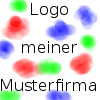
\includegraphics{images/firma-deckblatt.png}}}
	\end{longtable}
	\enlargethispage{20mm}
	\begin{center}
    \doublespacing{
		\vspace*{12mm}	{\LARGE\textbf \titel }}\\
		\vspace*{12mm}	{\large\textbf \arbeit}\\
		\vspace*{12mm}	\langdeckblattabschlusshinleitung\\
		\vspace*{3mm}		{\textbf \abschluss}\\
		\vspace*{12mm}	\langartikelstudiengang{} \langstudiengang{} \studiengang\\
    \vspace*{0mm}		\langanderdh{} \dhbw\\
		\vspace*{12mm}	\langvon\\
		\vspace*{3mm}		{\large\textbf \autor}\\
		\vspace*{12mm}	\datumAbgabe\\
	\end{center}
	\vfill
	\begin{spacing}{1.2}
	\begin{tabbing}
		mmmmmmmmmmmmmmmmmmmmmmmmmm             \= \kill
		\textbf{\langdbbearbeitungszeit}       \>  \zeitraum\\
		\textbf{\langdbmatriknr, \langdbkurs}  \>  \matrikelnr, \kurs\\
		\textbf{\langdbfirma}                  \>  \firma, \firmenort\\
		\textbf{\langdbbetreuer}               \>  \betreuer\\
		\textbf{\langdbgutachter}              \>  \gutachter
	\end{tabbing}
	\end{spacing}
\end{titlepage}

	\end{spacing}
	\newpage

	\pagenumbering{Roman}

	\pagestyle{plain}		% nur Seitenzahlen im Fuß
	
	\RedeclareSectionCommand[beforeskip=\kapitelabstand         ]{chapter} % stellt Abstand vor Kapitelüberschriften ein

	% Inhaltsverzeichnis
	\begin{spacing}{1.1}
		\begingroup
		
			% auskommentieren für Seitenzahlen unter Inhaltsverzeichnis
%%%			\renewcommand*{\chapterpagestyle}{empty}
%%%			\pagestyle{empty}
			
			
			\setcounter{tocdepth}{1}
			%für die Anzeige von Unterkapiteln im Inhaltsverzeichnis
			%\setcounter{tocdepth}{2}
			
			\tableofcontents
			\clearpage
		\endgroup
	\end{spacing}
	\newpage

	% Abkürzungsverzeichnis
	\cleardoublepage
%%%	%!TEX root = ../dokumentation.tex

\addchap{\langabkverz}
%nur verwendete Akronyme werden letztlich im Abkürzungsverzeichnis des Dokuments angezeigt
%Verwendung: 
%		\ac{Abk.}   --> fügt die Abkürzung ein, beim ersten Aufruf wird zusätzlich automatisch die ausgeschriebene Version davor eingefügt bzw. in einer Fußnote (hierfür muss in header.tex \usepackage[printonlyused,footnote]{acronym} stehen) dargestellt
%		\acs{Abk.}   -->  fügt die Abkürzung ein
%		\acf{Abk.}   --> fügt die Abkürzung UND die Erklärung ein
%		\acl{Abk.}   --> fügt nur die Erklärung ein
%		\acp{Abk.}  --> gibt Plural aus (angefügtes 's'); das zusätzliche 'p' funktioniert auch bei obigen Befehlen
%	siehe auch: http://golatex.de/wiki/%5Cacronym
%	
\begin{acronym}[YTMMM]
\setlength{\itemsep}{-\parsep}

\acro{AGPL}{Affero GNU General Public License}
\acro{WSN}{Wireless Sensor Network}
\acro{MANET}{Mobile wireless Ad-hoc NETwork}
\acro{MAC}{Multiple Access Control}
\acro{QoS}{Quality of Service}
\acro{DSR}{Dynamic Source Routing}
\acro{API}{Application Programming Interface}
\acro{WYSIWYG}{What You See Is What You Get}
\acro{HTML}{HyperText Markup Language}
\end{acronym}


	% Abbildungsverzeichnis
	\cleardoublepage
	\listoffigures

	%Tabellenverzeichnis
	\cleardoublepage
	\listoftables

	% Quellcodeverzeichnis
	\cleardoublepage
	\lstlistoflistings
	\cleardoublepage

	\pagenumbering{arabic}
	
	\pagestyle{headings}		% Kolumnentitel im Kopf, Seitenzahlen im Fuß

	% Inhalt
	%01Kapitel: Einfuehrung
	%02Kapitel: Struktur
	%03Kapitel: Layout
	%04Kapitel: Canvas Animationen
	%05Kapitel: AR Glasses
	%06Kapitel: Speech To Text Konvertierer
	
	%!TEX root = ../dokumentation.tex
\chapter{Einführung}
Wir leben in einer Zeit, in der der Einsatz von Technik im Alltag nicht mehr weg zu denken ist. Die Menschheit ist so stark vom technischen Fortschritt und den daraus resultierenden Entwicklungen geprägt wie nie zuvor.  
Technologien wie Autos, zu deren Betrieb eine körperliche Interaktion nicht mehr von Nöten ist, wurden vor wenigen Jahren noch als Science Fiction klassifiziert und sind trotz allem heute realisierbar. Auch In Fabriken werden selbst komplexere, erfolgsentscheidende Tätigkeiten von Robotern umgesetzt und zu Hause gehört das eigenständige Staubsaugen der Vergangenheit an, weil dies eine programmierte Maschine zuverlässig übernehmen kann. \\Neue Technologien wirken sich in vielen Alltagssituationen bereichernd und erleichternd auf unser Leben aus. Ein hiervon stark betroffener Wirtschaftssektor ist das wissens- und technologiegetriebene Gesundheitswesen. Der medizintechnische Fortschritt, der sich in den letzten Jahrzehnten ereignet hat, ermöglicht weitaus zielführendere Diagnose- und Therapiemöglichkeiten als sie früher vorstellbar waren. So lassen sich beispielsweise in der diagnostischen Fachabteilung Radiologie mit dem Einsatz neuer Technologien, wie Computer- und Kernspintomographien, aussagekräftigere Befunde erzielen als sie ein Pathologe früher durch einen händischen Eingriff hätte anfertigen können \cite[S.3]{buck_radiologie_2013}.\\Die Statistiken des statistischen Bundesamtes zur durchschnittlichen Lebenserwartung der Bevölkerung Deutschlands zeigen einen stetigen Aufschwung im Verlauf der vergangenen Jahrzehnte und lassen daher auf einen erheblichen Anstieg der allgemeinen Patientenversorgungsqualität im Gesundheitswesen aufgrund der Entwicklung IT-basierter Medizintechnologien schließen.\\ 
Diese Tatsache gilt als ausschlaggebender Beweggrund dafür, die Studienarbeit im Rahmen eines medizininformatischen Entwicklungsprojektes zu absolvieren. Der Fokus ist hierbei auf Menschen gerichtet, die von Hörschädigungen betroffen sind und tagtäglich mit ihren schwerwiegenden Folgen konfrontiert werden. Soziale Integrationsschwierigkeiten und psychische Beeinträchtigungen bilden nur das Grundgerüst der gängigen Symptomatik. Das Ziel des Projekts besteht darin, den oben genannten Belastungen durch Hörstörungen mithilfe eines IT-Produktes entgegenzuwirken.\\Als Entwicklungsgrundlage dient eine Technologie mit dem Namen Augmented Reality (zu Deutsch: Erweiterte Realität). Darunter lässt sich eine Variation der Ursprungstechnologie Virtual Reality verstehen, mit deren Hilfe Brillen entwickelt werden können, die dem User optisch das Gefühl vermitteln sich in einer virtuellen Welt zu befinden. Die reale Welt um ihn herum wird dabei vollständig ausgeblendet und ist für ihn somit nicht übersehbar.\\Augmented Reality (kurz: AR) sah dies als Schwachstelle und versuchte dem entgegenzuwirken. 
Durch AR lassen sich digitale Daten oder computergenerierte Informationen auf Brillen visualisieren und in die reale Welt integrieren. Gegenüber einer VR-Brille ist die reale Welt Teil der AR-Technologie und somit für den User sichtbar. AR erlaubt die Erfassung und Verarbeitung von Daten, beispielsweise die Aufzeichnung und Analyse eines gesehenen Bildes, und ermöglicht die Projizierung der Ergebnisse auf die Brillengläser \cite{kipper_augmented_2012}. Gleichermaßen lässt sich diese Konvertierung auch in die entgegengesetzte Richtung vornehmen, wie es auch im hier behandelten Studienprojekt verwendet wird:\\ 
Der von einem Mobiltelefon aufgenommene Ton wird auf das Vorkommen von Sprachbausteinen untersucht und die erkannte Sprache in Text konvertiert. Der Text wird auf einer AR-Brille ausgegeben, die in Verbindung mit dem Mobiltelefon steht. So kann ein Mensch auch mit Hörschädigungen einem Vortrag oder einer Unterrichtsstunde akustisch und visuell problemlos folgen. Auch das kommunizieren mit Menschen, die der Gebärdensprache nicht mächtig sind, wird vereinfacht, da diese einfach in das Mikrofon des Mobiltelefons sprechen müssen. Durch die Integration des Konvertierers in ein Mobiltelefon, wäre es sogar möglich beim Telefonat die Stimme des Anrufers direkt zu verarbeiten und dem Hörgeschädigten live als Text auf die AR-Brillengläser zu projizieren.


	%!TEX root = ../dokumentation.tex
\chapter{Struktur}
Die Applikation ist untergliedert in zwei Hauptbestandteile. Einen Recorder, welcher die Tonaufnahme durchführt und die erkannte Sprache in Text umwandelt, und ein Printer, welcher sich zu einer Augmenter Reality Brille verbindet und den vom Recorder erkannten Text forformatiert und darauf ausgibt. Das Bindeglied zwischen diesen beiden Komponenten ist das User Interface mit Klassenname MainActivity. Die MainActivity wird durch Usereingaben gesteuert. Sie erstellt bei bedarf neue Recorder oder Printer Instanzen, startet beziehungsweise stoppt die Aufnahme bzw die AR-Ausgabe und informiert den AR-Printer über neu verfügbare Ausgabetexte. Diese drei Komponenten werden im folgenden näher erleutert.

\section{Main Activity}
Wie bereits erwähnt ist die MainActivity das Zentrum der Applikation, ein UML-Klassendiagramm ist in XXX abgebildet.\\
Die bestandteile der MainActivity:
\begin{enumerate}
	\item Ein Spinner zur Wahl einer verfügbaren Sprachkonvertierungsoption und ein beschreibendes Textfeld
	\item Ein Spinner zur Wahl eines verfügbaren AR-Printers und ein beschreibendes Textfeld
	\item Ein Button zum Starten bzw. Stoppens einer Konvertierung
	\item Ein SideView Menü, welches Einstellungsmöglichkeiten enthält wie zum Beispiel das Festlegen der gesprochenen Sprache
	\item Eine Recorder Instanz vom Typ IRecorder. IRecorder ist ein interface, welches von allen Recorder-Implementierungen verwendet wird, um eine einheitlich API zu gewährleisten. Dieses Interface wird im Abschnitt XXX näher erleutert.
	\item Eine AR-Printer Instanz vom Typ IPrinter. Iprinter ist ebenfalls ein Interface, welches von allen AR-Printern zur Gewährleistung einer einheitlichen API implementiert wird und wird in Abschnitt XXX näher erleutert.
	\item Eine boolsche Hilfsvariable, die Auskunft darüber gibt, ob aktuell ein Konvertierungsvorgang im Gange ist.
	\item Zwei Integer-Variablen, die Auskunft über den aktuell gewählten Recorder bzw Printer geben.
\end{enumerate}
Zu 1. Und 2.:\\
Die beiden Spinner, enthalten alle aktuell supporteten Printer bzw Recorder. Der Inhalt der Spinner wird dynamisch genereiert, hierbei spielt die Klasse Constants eine tragende Rolle.\\
!!Genaueres über die initialisierung eines spinner arrays!!\\
Jedem der beiden Spinner ist eine OnItemSelectListener Instanz zugeordnet. Der OnItemSelectListener, ruft im Falle des Printer Spinners die Methode setPrinterMode(int mode, String description) und im Falle des Recorder Spinners die Methode setRecorderMode(int mode, String description) auf. Diese beiden Methoden initialisieren den gewünschten AR-Printer beziehungsweise den Recorder/Converter. Die Funktionalität dieser Methoden wird XXXX näher beschrieben.\\
Zu 3.:\\
Der OnClickListener der Buttons fragt die Hilfsvariable (7) ab und ruft abhängig von deren Wert die Methoden IRecorder.startRecording() und IPrinter.startPrinting() oder die Methode  notifyRecorderStop() der eigenen Klasse auf.\\
4. Menü: XXXX\par
Methoden der Klasse MainActivity:\\

onCreate() und initialize\_components():\\
In der onCreate()-Methode, welche beim start der Applikation ausgeführt wird, werden zunächst all Ihre bestandteile initialisiert durch die initialize\_components()-Methode.\\
setPrinterMode(int mode, String description)\\
Diese Methode prüft zuerst, ob im Moment ein Konvertierungsvorgang im Gange ist, durch das abfragen der boolschen Hilfsvariable isRecording. Im Falle einer laufenden Konvertierung wird eine Meldung ausgegeben, die den User darauf hinweißt, dass der AR-Printer während einer Konvertierung nicht gewechselt werden kann. Sonst wird nichts weiter unternommen.
Ist keine Konvertierung im Gange wird überprüft, ob der aktuelle Wert in der Hilfsvariable PRINTER\_MODE mit dem Wert des ausgewählten Printers in der übergebenen Variable mode übereinstimmt, denn auch dann muss keine weitere Aktion ausgeführt werden.\\
Wurde ein anderer Printer gewählt, als der gerade verwendete, wird die Methode generatePrinter(int mode, String description) der Klasse PrinterFactory aufgerufen. Die Methode generatePrinter prüft durch ein Switch Statement, welcher ARPrinter vom User gewünscht ist und gibt eine Instanz des gewünschten Printers and die aufrufende Methode zurück. Ist der übergebene Integer-Wert der Factory unbekannt, wird standardmäßig eine Instanz der Klasse TextPrinter erzeugt. Dieser erzeugt ein TextFeld in der MainActivity, in dem Speech to Text Conversion Ergebnisse ausgegeben werden.\\
setRecorderMode(int mode, String description):\\
Diese Methode hat den gleichen Ablauf, wie die Methode setPrinterMode(), mit dem einzigen Unterschied, dass die Methode generateRecorder der Klasse RecorderFactory aufgerufen wird, welche eine IRecorder Instanz zurück gibt. Auch die Recorder Factory hat für unbekannte Eingaben einen Standardwert. Sie gibt einen TextFieldRecorder zurück, welcher ebenfalls ein Textfeld erzeugt und die Eingaben and den gewählten AR-Printer sendet. Dieser Recorder verfehlt zwar den Sinn der Speech to Text Conversion, ist aber eine Erleichterung um die Funktionalität eines einzelnes AR-Printer Moduls zu testen.\\

receiveResult()\\
notifyStopRecord()\\

\section{Constants Klasse}
In der Klasse Constants werden globale Applikationskonstanten abgelegt. So gibt es für jede IRecorder-Implementierung einen Integer Wert, welcher den Recorder repräsentiert. Außerdem gibt es für jeden Recorder eine beschreibende String-Variable. Eine Map, welche beim start der Anwendung erzeugt wird, bringt die String-Werte mit den jeweiligen Int-Werten in Verbindung. Analog dazu besteht die selbe Struktur für Instanzen des Typs IPrinter, die unterstützten AR-Printer verwalten zu können.


\section{Interface für AR-Glass-Printer}
\section{Interface für Speech-To-Text-Konvertierer}

	%!TEX root = ../dokumentation.tex
\chapter{Graphical User Interfaces}

	\section{ActionBar}
	\section{NavigationView als Sidebar}
	\section{Buttons / Buttondesigning}
	\section{Spinner}
	\section{TextViews}
	\section{EventListener}
	\section{SurfaceView für Animation}
	%!TEX root = ../dokumentation.tex
\chapter{Canvas Animationen}

\section{Dummy}
	%!TEX root = ../dokumentation.tex
\chapter{AR-Glass-Printer Implementierungen}

\section{Die Klasse AbstractPrinter}
\section{Support der GlassUp AR Brille}
\section{Der TextField Printer}
	%!TEX root = ../dokumentation.tex
\chapter{Speech-To-Text-Konvertierung}


\section{Der Android Speech Recognition Client}


\section{Speech-To-Text Konvertierung durch die Google Cloud API}
\paragraph{Aufbau des Moduls}
Die Klassen des Google Speech Recognition Moduls befinden sich im package de.dhbw.studienarbeit.hearItApp.recorder.googleSpeechRecognition. Zum aufzeichnen des Tons dient die Klasse VoiceRecorder welche das in XXX beschriebene IRecorder Interface implementiert. Die Klasse VoiceRecorder wird der Klasse MainActivity als Recorder Instanz zugeordnet, wenn im User Interface die Google Speech Recognition als Option gewählt wurde. Sie implementiert die Interface Methoden startRecording(), stopRecording() und shutdown(). In ihrem Konstruktor wird die Klasse GoogleSpeechConverter instanziiert. Diese Klasse ist verantwortlich für die Konvertierung der vom VoiceRecorder aufgenommenen Audiodaten. Sie kommuniziert mit den Google Servern, sendet Audiodaten und empfängt das Konvertierungsergebnis.\\
Diese Komponenten werden im folgenden näher erläutert.
\\

\subsection{Der Voice Recorder}
Zur Aufnahme von Ton bietet Android zwei Optionen\cite{Recording Optionen}:
\begin{enumerate}
	\item Die Erste ist der Android Media Recorder. Dieser bietet ein einfaches Interface, um mit wenigen Code Zeilen eine Audio Aufnahme zu starten und die Audio Daten in eine Datei zu schreiben. Nach beendigung der Aufnahme kann die Datei abgespielt oder weiter verarbeitet werden.
	\item Die Zweite und für diesen Zweck passendere Methode ist die Audio Aufnahme durch ein Objekt der Klasse AudioRecord. Die Programmierung des AudioRecords findet eine Ebene tiefer statt, als die des MediaRecorders. Nachdem dem Objekt durch den Konstruktor die Aufnahmequelle, das Sampling, die Anzahl der Channels, das Encoding und die Buffergröße zugewiesen wurden, können nach dem Starten der Aufnahme in einer Schleife die aufgenommenen Audio Daten in Form von Byte oder Short Arrays ausgelesen werden.
\end{enumerate}
Ein Code-Beispiel zur Initialisierung und Aufnahme durch ein AudioRecord Objekt sieht so aus:
\begin{lstlisting}
AudioRecord androidRecord = new AudioRecord(MediaRecorder.AudioSource.MIC,
		VoiceRecorder.SAMPLING, VoiceRecorder.RECORDER_CHANNELS,
		VoiceRecorder.RECORDER_AUDIO_ENCODING, VoiceRecorder.BUFFER_SIZE);
		
androidRecord.startRecording();
boolean isRecording = true;

while (isRecording) {

	short[] shortBuffer = new short[VoiceRecorder.BUFFER_SIZE / 2];
	
	//read ist return code, shortBuffer der Buffer in den geschrieben wird
	int read = this.androidRecord.read(shortBuffer, 0, shortBuffer.length);
	
	//verarbeite auio daten in shortBuffer
	
}
\end{lstlisting}

\paragraph{Begrifflichkeiten}
Die im Konstruktor übergebenen Daten sind die Audioquelle, das Sampling, die Anzahl der Channels, das Encoding und die Buffergröße.\\
Die Audio Quelle ist das Gerät, von welchem Ton aufgezeichnet werden soll und die Anzahl der Channels gibt an, über wie viele Kanäle der Ton aufgenommen wird (Mono, Stereo, usw).\\
Unter dem Sampling versteht man die Anzahl der Werte die pro Sekunde aus dem Analogen Signal einer Audioquelle entommen werden sollen. Weil ein Analoges Signal eine Welle bestehend aus unendlich vielen Werten darstellt, muss das Signal zur digitalen Speicherung auf eine definierte Punktezahl reduziert werden. Diese Zahl nennt sich Sampling. Für dieses Projekt wurde ein 16 000 Sampling gewählt, da ein Kompromiss zwischen Übertragungszeit und Qualität gefunden werden musste. Je höher das Sampling, umso größer die Daten Menge, umso höher die Übertragungszeit.\\
Das Encoding gibt die Zahl der Bits an, die jeder gespeicherte Wert hat. Bei einem 16 Bit Encoding, hat jeder gespeicherte Wert eine größe von 2 Byte.\\
Die Buffergröße ist die Größe des Arrays, in welchen man die Daten später einliest. Die Buffergröße gibt an, wie viele Sekunden jeweils vom Mikrophon ausgelesen werden sollen.\\
Herleitung Buffer Größe:\\
Pro Schleifendurchlauf sollen 80 aufgezeichnete Millisekunden vom AudioRecord gelesen werden.\\
Ein Sampling von 16 000 mit Encoding 16 Bit, bedeutet, dass pro Sekunde 16 000 Werte a 16 Bit gespeichert werden, was 16 000 Werten von je 2 Byte also 32 000 Byte = 32 kByte enstspricht. Multipliziert man diesen Wert mit der gewünschten Aufnahme Zeit ergibt sich die Größe eines Buffers in Byte.\\
Die Speichergröße errechnet sich dann wie folgend:\\
\begin{equation}
Speichergröße = Sampling  * \frac{Encoding}{8} * Zeit \\
Speichergröße = 16 000 	  * \frac{16}{8} 	  * 0,8  = 25 600 Byte
\end{equation}
Nun kann also entweder ein Byte Array mit größe 25 600 an den AudioRecord übergeben werden, oder aber ein Short Array mit der halben größe, da  ein Short-Wert eine größe von 2 Byte hat.\\

\paragraph{Funktionaler Aufbau des Voice Recorders}
Nachdem die Option Google Speech Conversion im User Interface gewählt wurde, wird durch die RecorderFactory Klasse eine Instanz des VoiceRecorders erzeugt. Im Konstruktor werden sowohl ein AudioRecord Objekt, als auch ein GoogleSpeechConverter Objekt, welches im Verlauf noch näher erläutert wird, inizialisiert. Danach steht der Recorder zur Verwendung bereit. \\
Wird im User Interface der Button zum starten der Konvertierung gedrückt, ruft die Klasse MainActivity die Methode startRecording() des Recorders auf. Innerhalb dieser Methode wird die Methode readAudioInput() der eigenen Klasse in einem eigenen Thread gestartet.\\
ReadAudioInput() setzt das Attribut isRecording auf true und beginnt eine while-Schleife, mit isRecording = false als Abbruchskriterium. Innerhalb der Schleife wird pro Durchlauf ein AudioBuffer mit Audio Daten gefüllt. Der Audio Buffer ist vom Typ short[]. Dieser Buffer wird der MainActivity-Methode showSoundAnimation übergeben, welche in Abhängigkeit der aus den Daten errechneten Lautstärke eine Animation erzeugt, um die laufende Aufnahme für den Benutzer zu visualisieren.\\
Danach wird  der short[]-Buffer durch die Methode convertShortToByte[] in einen byte[]-Buffer konvertiert und der Methode recognizeBytes der Klasse GoogleSpeechConverter übergeben, welche die Daten an Google sendet, um gesprochene Sprache zu erkennen und diese in Text zu konvertieren.\\
Die Konvertierung von short zu byte ist notwendig, da die Google Streaming Speech API lediglich byte[]-Buffer als Übergabewert akzeptiert. Die Methode showSoundAnimation verwertet allerdings short-Werte, da bei einem 16-Bit Encoding jeder einzelne Audiowert die länge von 2 byte, also einer short hat. Bei der Konvertierung wird jeder short-Wert im Buffer einmal mit 0x00FF maskiert  und das Ergebnis in einen byte-Array geschrieben. Die Maske 0x00FF setzt die oberen 8 Bit auf 0 und übernimmt die Werte der untern 8 Bit. Es bleibt eine 1 Byte große Zahl, welche den Wert der unteren Hälfte der short-Zahl hat. Danach wird die short-Zahl mit >> 8 um 8 Bit nach rechts geshiftet. Dies hat zur Folge, dass die untern 8 Bit verschwinden, während die oberen 8 Bit an die untere Stelle rücken. Die oberen 8 Bit werden mit nullen aufgefüllt. Wieder bleibt eine 8 Bit lange Zahl, welche die Werte der oberen Hälfte der short-Zahl enthält. Diese wird an die darauf folgende Stelle im byte-Buffer geschrieben.\\
Es entsteht ein Array der Form:
\begin{addmargin}[1cm]{0cm}
	buffer[0] = low Nibble Short[0]
	buffer[1] = high Nibble Short[0]
	buffer[2] = low Nibble Short[1]
	buffer[3] = high Nibble Short[1]
	...
\end{addmargin}
Quellcode der convertShortToByte-Methode:
\begin{lstlisting}
private byte[] convertShortToByte(short[] buffer) {

	byte[] byteBuffer = new byte[buffer.length * 2];

	for (int i = 0; i < buffer.length; i++) {
		//mask to set high 8 bit of short 0, let low 8 bit as is, add to array
		byteBuffer[i * 2] = (byte) (buffer[i] & 0x00FF);
		//shift right to get high 8 bit down, and add high bits to array
		byteBuffer[(i * 2) + 1] = (byte) (buffer[i] >> 8);
	}
return byteBuffer;

}
\end{lstlisting}
Wird der UI-Button zum Stoppen der Aufnahme gedrückt, oder passiert im Connector, GoogleSpeechConverter oder Recorder selbst ein schwerwiegende Fehler, wird die Recorder-Methode stopRecording() ausgeführt. Diese Methode Methode setzt das Attribut isRecording auf false, was zur Beendigung der Schleife führt. Auserdem wird die Methode stop() des AudioRecord Objektes ausgeführt, welche den Aufnahmevorgang stoppt.\\
Innerhalb der shutdown() Methode, welche beim Wechsel der Aufnahmemethode zu einem anderen Recorder-Modul aufgerufen wird, werden vom AudioRecord belegte Resourcen durch die Methode release() wieder frei gegeben.
\subsection{Der Google Speech Converter}
Der GoogleSpeechConverter ist der mit der Google Speech API kommunizierende Modulteil. Er sendet Audio Daten und empfängt die Konvertierungsergebnisse, welche er dann an die MainActivity Klasse weitergibt, die diese an einen AR-Connector weiterleitet. Um den Aufbau der GoogleSpeechConverter Klasse darzustellen wird im folgenden zunächst die API der Google Cloud Funktion für Sprachkonvertierung erläutert. Im Anschluss wird auf die Implementierung innerhalb der Applikation eingegangen. 

\paragraph{Die Google Cloud Speech API}
Zum Zugriff auf die Google Cloud Speech API bestehen drei Möglichkeiten \cite{API Doc}:
\begin{enumerate}
	\item Synchrone Konvertierung\\
	Im ersten Fall wird eine Audiodatei an Google gesendet, welche konvertiert wird. Erst nach Abschluss des Konvertierungsvorgangs erhält der Client eine Antwort in Form eines JSON Strings, welcher den erkannten gesprochenen Text enthält.
	\item Asynchrone Konvertierung\\
	Im zweitenen Fall, der asynchronen Konvertierung werden dem Client Teilergebnisse der Konvertierung der gesendeten Audiodatei schon mitgeteilt, sobald diese verfügbar sind und nicht erst nach Abschluss der Konvertierung.
	\item Konvertierung durch Live Streaming\\
	Weil im Falle der hier thematisierten Applikation keine Audio Datei zur Verfügungn steht, sondern ein in echtzeit vom Mikrophon aufgenommener Audiostream, wird hier von der dritten Möglichkeit, der Live Streaming Variante gebrauch genommen. Bei dieser Option, sendet ein Client Audiopakete über einen Http-Stream an Google und empfängt über einen Antwort-Stream die Teilergebnisse der bisher konvertierten Daten.\\
	Die Audiodaten müssen hierfür in nahezu Echtzeit gesendet werden. Dies bedeutet, dass in jeder Sekunde nach Start der Konvertierung, Audiodaten einer Sekunde beim Google Server eingegangen sein müssen. Dies macht deutlich, dass die Übertragungsgeschwindigkeit hierbei eine große Rolle spielt. Werden vom Client im Abstand von 0,5 Sekunden Audiopakete mit Audiodaten der letzen 0,5 Sekunden gesendet, diese Pakete benötigen allerdings, aufgrund schlechter Übertragunsgeschwindigkeit 4 Sekunden zur Übertragung, erhält der Google Server lediglich alle 4 Sekunden Audio Daten von 0,5 Sekunden, wojdurch ein Konvertieren nicht mehr möglich ist.
\end{enumerate}
\paragraph{Authentifizierung bei der Google Speech API}
Laut Googles API Dokumentation ist die sicherste Variante der Authentifizierung bei der Google Cloud die Authentifizierung durch einen Service Account. \cite{ https://cloud.google.com/speech/docs/common/auth}. Ein Service Account ist ein Google Account, über den durch Apps Google Services genutzt werden können. Zur Authentifizierung bei einem Account dient ein asynchrones Private-Public-Key-Verfahren. Nachdem Anlegen des Accounts, genereiert ein Entwickler zunächst ein Service Account Key-Paar in Form von JSON Strings. Der Key kann für eine oder mehrere Google APIs zugelassen werden. Im Falle dieses Projekts wurde er auf die Speech API beschränkt um Missbrauch zu vermeiden. Der JSON String wird als Datei im Projekt hinterlegt. Bei der Authentifizierung generiert Google ein syncrones Auth-Token, welches in der weiteren Kommunikation zur Identifikation des Authotisierten Clients.\\

\paragraph{OAuth Authentifizierung in Java}
Der sich authentifizierende Client verwendet einen InputStream um den im Projekt hinterlegten Key einzulesen. Er initialisiert ein Objekt der Klasse GoogleCredentials, welche im Package com.google.auth.oauth2 der Library com.google.auth:google-auth-library-oauth2-http:0.3.0 zu finden ist, und weißt ihm den Key-String zu. Dem GoogleCredentials Objekt wird ein Scope hinzugefügt, also ein Ziel, für welches die Credentials bestimmt sind. In diesem Fall ist das https://www.googleapis.com/auth/cloud-platform.\\
Durch die Klasse OkHttpChannelProvider und OkHttpChannelBuilder der Library io.grpc:grpc-okhttp, kann ein ManagedChannel Objekt erzeugt werden, welchem das zuvor generierte GoogleCredentials als parameter hinzugefügt wird. Das Objekt der Klasse ManagedChannel abstrahiert die Authentifizierung bei Google und stellt eine Verbindung zur Google API her. Jede Kommunikation mit der API erfolgt über diesen Channel.

\paragraph{Die Google Speech RPC API}
Zum Zugriff auf Funktionen der Speech API, werden zwei Optionen Angeboten: Zugriff via REST und Zugriff via RPC. Da die REST API nur für non-Streaming Use Cases verwendet werden kann, wird in diesem Projekt von der RPC API gebrauch gemacht \cite{https://cloud.google.com/speech/docs/apis}. Zugriffe über das Remote Procedure Call Protokoll bieten sich in diesem Fall an, da durch Remote Procedures bidirektionales Streaming ermöglich wird, während ein Client bei REST Zugriffen nach dem senden einer Http-Anfrage so lange wartet, bis eine Antwort eintrifft. Für Streaming während in festen Abständen immer wieder neue Audiodaten gesendet werden, ist es wichtig, dass die Antworten über einen zweiten Stream asynchron empfangen werden können. Auf RPC Methoden der Google Speech Cloud kann in Java durch die Library google.cloud.speech.v1beta1 zugegriffen werden. Die RPC Schnittstelle von Google wird auch gRPC API genannt \cite{tps://cloud.google.com/speech/docs/apis}.\\
Folgende Funktionen werden von der RPC API angeboten:\\
\begin{enumerate}
	\item Das Interface Speech definiert, dass eine rpc Anfrage StreamingRecognize mit einem StreamingRecognizeRequest als Anfrage mit einem StreamingRecognizeResponse Objekt antwortet.
	\item Um eine StreamingRecognize Anfrage zu stellen, muss ein StreamingRecognizeRequest Objekt erzeugt werden. Diesem Objekt wird entweder ein Parameter streaming\_config oder audio\_config hinzugefügt.
	\item Im ersten StreamingRecognizeRequest müssen der API die Attribute der Gesendeten Audiodaten mitgeteilt werden. Dies geschieht durch ein StreamingRecognitionConfig Objekt, welches dem StreamingRecognizeRequest hinzugefügt wird.\\
	Das StreamingRecogntitionConfig Objekt enthält ein RecognitionConfig Objekt, in welchem Informationen über das verwendete Encoding, Sampling und die Sprache gespeichert sind. Außerdem wird durch die boolschen Parameter single\_utterance und interim\_results definiert, ob die Konvertierung bei einer Sprechpause beendet werden soll und ob auch geratene Ergebnisse mitgeteilt werden sollen. Geratene Ergebnisse entstehen während der Konvertierung einer Phrase, bevor deren Ende noch nicht erreicht ist. Geratene Ergebnisse sind zu einer mitgesendeten Wahrscheinlichkeit korrekt. Endgültige Ergebnisse haben eine Sicherheit von 98+ %.
	\item Alle weiteren StreamingRecognizeRequests enthalten nur noch audio\_content, in Form eines byte Arrays von Audio Daten, welchen im zuvor spezifizierten Format codiert sind.
	\item Auf jede StreamingRecognize Anfrage antwortet der Server mit einem StreamingRecognizeResponse Objekt in einem gesonderten Stream. Die StreamingRecognizeResponse ist ein JSON String. Dieser kann Flags zum hinweis auf den Beginn oder die Beendigung der Konvertierung enthalten. Innerhalb einer Konvertierung enthält der String ein oder mehrere alternatives Objekte. Diese bestehen aus einem "transcript"-Wert, also einer Übersetzung und einer "stability", also der Wahrscheinlichkeit mit der die Übersetzung korrekt ist. Die alternatives Objekte sind in absteigender Wahrscheinlichkeit sortiert.\\
	ein is\_final: true flag gibt an, dasss die Übersetzte Phrase nun final übersetzt wurde und sich nicht mehr ändert. Setzt man alle Ergebnisse, die dieses Flag enthalten zusammen, erhält man das Gesamtergebnis. Wurde der interim\_results Parameter innerhalb der RecognitionConfig auf false gesetzt, werden nur finale Ergebnisse mitgeteilt.
\end{enumerate} \cite{https://cloud.google.com/speech/reference/rpc/google.cloud.speech.v1beta1}

\paragraph{Implementierung des Google Speech API Zugriffes}
Die Funktionen bezüglich des Zugriffs auf die Google Speech API sind in der Klasse GoogleSpeechConverter im package de.dhbw.studienarbeit.hearItApp.recorder.googleSpeechRecognition gebündelt.
Der zuvor bereits thematisierte VoiceRecorder ruft im Konstruktor die private Methode initializeSpeechConverter() auf. 
Innerhalb dieser Methode wird eine neue Instanz des GoogleSpeechConverters erzeugt und dem VoiceRecorder als Attribut hinzugefügt.\\
Im Konstruktor des GoogleSpeechConverters wird ein Thread gestartet, welcher ständig die aktuelle Übertragungsgeschwindigkeit überprüft, da bei einer zu kleinen Geschwindigkeit keine Konvertierung stattfinden kann, weil Audiodaten in Echtzeit gestreamt werden müssen.\\
Danach wird durch die Methode createChannel() ein ManagedChannel nach dem bereits beschriebenen Ablauf erzeugt.
\begin{lstlisting}
 private Channel createChannel()
 	throws IOException, GeneralSecurityException {
 	
	InputStream credentials =this.recorder.getMainView()
		.getAssets().open(authentication\_key);
		
	GoogleCredentials creds = GoogleCredentials.fromStream(credentials)
		.createScoped(this.OAUTH2\_SCOPES);
		
	OkHttpChannelProvider provider = new OkHttpChannelProvider();
	OkHttpChannelBuilder builder = provider.builderForAddress(
		this.HOST, this.PORT);
	
	ManagedChannel channel = builder.intercept(
		new ClientAuthInterceptor(
		creds, Executors.newSingleThreadExecutor()))
		.build();
	
	credentials.close();
	
	return channel;
}
\end{lstlisting}
Mit diesem Channel wird ein SpeechGrpc.SpeechStub Objekt initialisiert durch die Methode SpeechGrpc.newStub(channel).\\
Wird dann eine Aufnahme gestartet, ruft der VoiceRecorder nach jedem lesen von AudioBytes die Methode recognizeBytes(byte[] buffer, int size) auf.\\
Innerhalb dieser Methode erfolgt eine Überprüfung, ob der Converter bereits initialisiert wurde. Wenn nicht, wird die Methode initializeStreaming() aufgerufen. Hier wird dem im Konstruktor initialisierten SpeechStub durch die Methode speechRPCStub.streamingRecognize(this) der ResponseStreamObserver zugewiesen.\\
Der Zugewiesene ResponseStreamObserver wird vom SpeechStub benachrichtigt, sobald eine Antwort von der SpeechAPI erhalten wird. Um als solcher zu funkieren, muss die Klasse das Interface io.grpc.stub.StreamObserver<StreamingRecognizeResponse> und die zugehörigen, selbsterklärenden Methoden onNext(StreamingRecognizeResponse response), onError( Throwable error ) und onCompleted() implementieren. Diese Methoden werden im jeweiligen Fall vom SpeechStub aufgerufen.\\
Die Methode speechRPCStub.streamingRecognize(this) gibt ein Objekt der Klasse StreamObserver<StreamingRecognizeRequest>, welches im Attribut requestObserver gespeichert wird, zurück. Über den RequestObeserver Stream können Daten an die Google API gesendet werden.\\
Sind beide Streams initialisiert, wird nach den zuvor beschriebenen API Regeln eine RecognitionConfig in eine StreamingRecognitionConfig eingebettet und daraus ein StreamingRecognizeRequest erzeugt, welches durch die Methode requestObserver.onNext(requehst) an die API gesendet wird, um die Konvertierung zu initialisieren. Der Programmcode zum generieren der Konfiguration ist im Anschluss abgebildet.
\begin{lstlisting}
RecognitionConfig audioConfig =
	RecognitionConfig.newBuilder()
		.setEncoding( RecognitionConfig.AudioEncoding.LINEAR16 )
		.setSampleRate( VoiceRecorder.SAMPLING )
		.build();

StreamingRecognitionConfig streamingConfig =
	StreamingRecognitionConfig.newBuilder()
		.setConfig( audioConfig )
		.setInterimResults( false )
		.setSingleUtterance( false )
		.build();

StreamingRecognizeRequest initialRequest =
	StreamingRecognizeRequest
		.newBuilder()
		.setStreamingConfig( streamingConfig )
		.build();
		
//send initial request with config
this.requestObserver.onNext(initialRequest);

\end{lstlisting}
Nachdem die Konvertierung nun initialisiert wurde, wird in der recognizeBytes Methode das isInitialized Flag auf true gesetzt, um eine erneute Initialisierung zu vermeiden.\\
Um die Audio Daten zu Google zu senden, wird erneut ein StreamingRecognizeRequest initialisiert. Statt einer StreamingRecognitionConfig, werden diesem aber durch die Methode setAudioContent die Übergebenen Audio Bytes zugewiesen. Durch requestObserver.onNext(request) wird der Request gesendet.

\begin{lstlisting}
public void recognizeBytes(byte[] buffer, int size){

	if (!this.isInititalized) {
		this.initializeStreaming();
		this.isInititalized = true;
	}
	try {
		StreamingRecognizeRequest request =
			StreamingRecognizeRequest.newBuilder()
				.setAudioContent(ByteString
					.copyFrom(buffer, 0, size))
				.build();
		requestObserver.onNext(request);
		
	} catch (RuntimeException e){
		Log.e(MainActivity.LOG\_TAF, "Error while recognizing speech. Stopping."
			+ e.getMessage());
		requestObserver.onError(e);
		throw e;
	}
}

\end{lstlisting}

\paragraph{Verarbeitung der Antworten}
Die Verarbeitung der Antworten, passiert im dem SpeechStub zugewiesenen ResponseStreamObserver, welcher ebenfalls in der GoogleSpeechConverter Klasse implementiert ist.\\
Bei einem Fehler wird die onError Methode mit einem Throwable als Parameter aufgerufen. Innerhalb der Methode, wird der Fehler in die Log Datei geschrieben und durch this.recorder.stopRecording() die Aufnahme beendet.\\
Bei einem positiven Ergebnis wird innerhalb der aufgerufenen onNext(StreamingRecognizeRespone respone) Methode die Liste der in der response entahltenen StreamingRecognitionResults ausgelesen. Sind Ergebnisse in der Antwort enthalten, werden vom ersten Ergebnis, welches den Index 0 hat, durch getAlternativesList() die Übersetzungsalternativen gewonnen. Die erste alternative, die die Wahrscheinlichste Übersetzung darstellt, wird durch this.recorder.getMainView().receiveResult(alternative.getTranscript()) and die MainActivity weiter geleitet, welche den ausgewählten Connector mit der Anzeige des Textes beauftragt.\\
Eine Prüfung des is\_final Flags in der Antwort ist nicht notwendig, da durch das setzen der Einstellung interrim\_results=true während der Initialisierung des Streamings sichergestellt wurde, dass alle Antworten nur finale Phrasen enthalten.


\paragraph{Überprüfung der Übertragungsgeschwindigkeit}

\paragraph{Zeitliche Analyse der Konvertierung}
\paragraph{Maximaler Streaming Zeitraum}


\section{Der TextFieldRecorder / Konvertierer}
	
%	\foreach \i in {01,02,03,04,05,06,07,08,09,...,99} {%
%		\edef\FileName{content/\i kapitel}%
%			\IfFileExists{\FileName}{%
%				\input{\FileName}
%			}
%			{%
				%file does not exist
%			}
%	}

	\clearpage

	% Literaturverzeichnis
	\cleardoublepage
	\printbibliography

	% Glossar
	\printglossary[style=altlist,title=\langglossar]
	
	% sonstiger Anhang
	\clearpage
	\appendix
	% !TeX root = ../dokumentation.tex

\addchap{\langanhang}

(Beispielhafter Anhang)
 

{\Large
\begin{enumerate}[label=\Alph*.]
	\item Assignment 
	\item List of CD Contents
	\item CD 
\end{enumerate}
}
\pagebreak
%\includepdf[pages=-,scale=.9,pagecommand={}]{Aufgabenstellung.pdf} % PDF um 10% verkleinert einbinden --> Kopf- und Fußzeile  werden so korrekt dargestellt. Die Option `pages' ermöglicht es, eine bestimmte Sequenz von Seiten (z.B. 2-10 oder `-' für alle Seiten) auszuwählen.
\pagebreak
\section*{B. Auflistung der Begleitmaterial-Archivdatei }
Die Archivdatei wurde zusammen mit der Online-Version dieser Ausarbeitung auf die Lernplattform hochgeladen.
\begin{tabbing}
	mm \= mm \= mmmmmmmmmmmmmmmm \= \kill
	$\vdash$ \textbf{Literature/} \\ 
	| \> $\vdash$ \textbf{Citavi-Project(incl pdfs)/} \> \> $\Rightarrow$ \textit{Citavi (bibliography software) project with}\\
	| \> | \> \> \textit{almost all found sources relating to this report.} \\
	| \> | \> \> \textit{The PDFs linked to bibliography items therein} \\
	| \> | \> \> \textit{are in the sub-directory `CitaviFiles'}\\
	| \> | \>  -- bibliography.bib  \> $\Rightarrow$ \textit{Exported Bibliography file with all sources}\\
	| \> | \>  --	Studienarbeit.ctv4  \>  $\Rightarrow$ \textit{Citavi Project file}\\
	| \> | \>  $\vdash$ \textbf{CitaviCovers/} \>  $\Rightarrow$ \textit{Images of bibliography cover pages}\\
	| \> | \>  $\vdash$ \textbf{CitaviFiles/} \> $\Rightarrow$ \textit{Cited and most other found PDF resources}\\ %\llcorner
	| \> $\vdash$ \textbf{eBooks/} \\
	| \> $\vdash$ \textbf{JournalArticles/} \\
	| \> $\vdash$ \textbf{Standards/}\\
	| \> $\vdash$ \textbf{Websites/} \\ %\llcorner
	|\\
	$\vdash$ \textbf{Presentation/} \\
	| \>  --presentation.pptx\\
	| \>  --presentation.pdf\\
	|\\
	$\vdash$ \textbf{Report/} \\ %\llcorner
	\>  -- Aufgabenstellung.pdf\\
	\>  -- Studienarbeit2.pdf\\
	\>  $\vdash$ \textbf{Latex-Files/}   $\Rightarrow$ \textit{editable \LaTeX~files and other included files for this report}\\ %\llcorner
	\> \>  $\vdash$  \textbf{ads/}   	\> $\Rightarrow$ \textit{Front- and Backmatter}\\
	\> \>  $\vdash$  \textbf{content/}  \> $\Rightarrow$ \textit{Main part}\\
	\> \>  $\vdash$  \textbf{images/}   \> $\Rightarrow$ \textit{All used images}\\
	\> \>  $\vdash$  \textbf{lang/}  \> $\Rightarrow$ \textit{Language files for \LaTeX~template}\\ %\llcorner
\end{tabbing}

	
\end{document}
